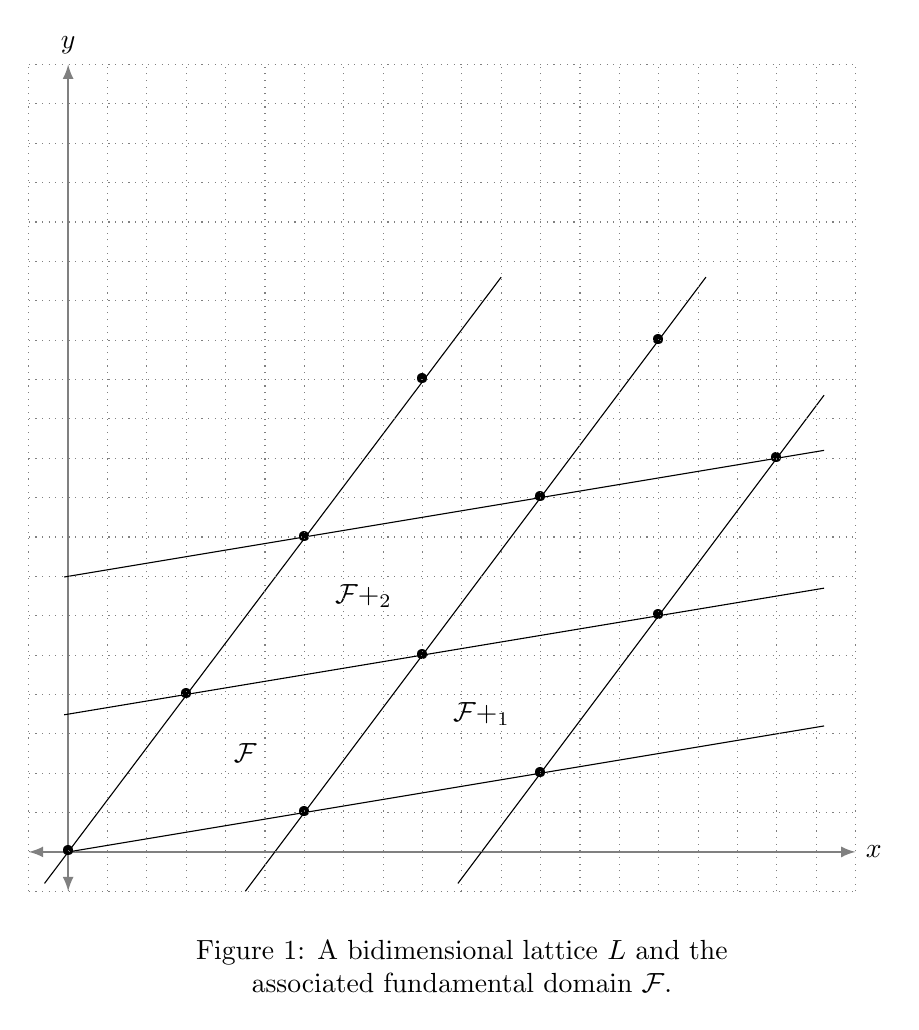
\begin{tikzpicture}[scale = 0.5]
\draw[latex-latex, thick, draw=gray] (-1,0)--(20,0) node [right] {$x$}; 
\draw[latex-latex,thick, draw=gray] (0,-1)--(0,20) node [above] {$y$};

\foreach \Point in {(0, 0), (3, 4), (6,1), (9, 5), (6, 8), (9, 12), (12, 9), (15, 13), (12,2), (15, 6), (18, 10)}{
	\node at \Point {\textbullet};
}

\draw[black] (-0.6, -0.8) -- (11, 14.6);
\draw[black] (4.5, -1) -- (16.2, 14.6);
\draw[black] (9.9, -0.8) -- (19.2, 11.6);

\draw[black] (-0.1, -0.0166) -- (19.2, 3.2);
\draw[black] (-0.1, 3.483333) -- (19.2, 6.7);
\draw[black] (-0.1, 6.983333) -- (19.2, 10.2);


\node [black] at (4.5,2.5) {$\mathcal{F}$};
\node [black] at (10.5,3.5) {$\mathcal{F}+ \vv_1$};
\node [black] at (7.5,6.5) {$\mathcal{F}+ \vv_2$};
\draw [dotted, gray] (-1,-1) grid (20,20);

\node [below=1cm, align=flush center,text width=8cm] at (10, 0)
{
	Figure 1: A bidimensional lattice $L$ and the associated fundamental domain $\mathcal{F}$.
};
\end{tikzpicture}